
\documentclass[idxtotoc,hyperref,openany,oneside]{labbook} % 'openany' here removes the gap page between days, erase it to restore this gap; 'oneside' can also be added to remove the shift that odd pages have to the right for easier reading

\usepackage[ 
  backref=page,
  pdfpagelabels=true,
  plainpages=false,
  colorlinks=true,
  bookmarks=true,
  pdfview=FitB]{hyperref} % Required for the hyperlinks within the PDF
  
\usepackage{booktabs} % Required for the top and bottom rules in the table
\usepackage{float} % Required for specifying the exact location of a figure or table
\usepackage{graphicx} % Required for including images
\usepackage{lipsum} % Used for inserting dummy 'Lorem ipsum' text into the template

\newcommand{\HRule}{\rule{\linewidth}{0.5mm}} % Command to make the lines in the title page
\setlength\parindent{0pt} % Removes all indentation from paragraphs

%----------------------------------------------------------------------------------------
%	DEFINITION OF EXPERIMENTS
%----------------------------------------------------------------------------------------

\newexperiment{example}{This is an example experiment}
\newexperiment{example2}{This is another example experiment}
\newexperiment{example3}{This is yet another example experiment}
\newexperiment{table}{This shows a sample table}
%\newexperiment{shorthand}{Description of the experiment}

%---------------------------------------------------------------------------------------

\begin{document}

%----------------------------------------------------------------------------------------
%	TITLE PAGE
%----------------------------------------------------------------------------------------

\frontmatter % Use Roman numerals for page numbers
\title{
\begin{center}
\HRule \\[0.4cm]
{\Huge \bfseries Laboratory Journal \\[0.5cm] \Large Master of Science}\\[0.4cm] % Degree
\HRule \\[1.5cm]
\end{center}
}
\author{\Huge Serhii Volosheniuk \\ \\ \LARGE Volosheniuk.Serhiy@gmail.com \\[2cm]} % Your name and email address
\date{Beginning 1 February 2018} % Beginning date
\maketitle

\tableofcontents

\mainmatter % Use Arabic numerals for page numbers

%----------------------------------------------------------------------------------------
%	LAB BOOK CONTENTS
%----------------------------------------------------------------------------------------

% Blank template to use for new days:

%\labday{Day, Date Month Year}

%\experiment{}

%Text

%-----------------------------------------

%\experiment{}

%Text

%----------------------------------------------------------------------------------------

\labday{1-12 February 2018, Sample preparation}

\experiment{mesa-structure}
hey how are you

%-----------------------------------------

\experiment{Gate} % Multiple experiments can be included in a single day, this allows you to segment what was done each day into separate categories

\begin{figure}[H] % Example of including images
\begin{center}
%\includegraphics[width=0.5\linewidth]{example_figure}
\end{center}
\caption{Example figure.}
\label{fig:example_figure}
\end{figure}

%-----------------------------------------

\experiment{Contacts}
here i 'm going to wright something

%----------------------------------------------------------------------------------------

\labday{13-25 February 2018, Transport measurements HgTe}
\experiment{Some theory notes}
In order to calculate $\rho_x$ we need to know geometrical parametr. In our case $\frac{S}{l}=0.176$
\experiment{Transport analysis}
In order to check our sample we have done transport measurements. The sample is putted into Cryogenic Transport Measurement System(CFMS) and field dependancies of Rxx and Rxy are measured with different temperatures. 
In the fig1. the scheme of sample contacts is presented. Current is aplied to contuct  3 and 4 via resistor 1MOhm, the lockin voltage is 0.5V. We measure Rxx between contucts  1 and 2, Rxy  between  1 and 6. 
Temperature dependence of Rxx and Rxy are presented in fig2.
(Here will be tex about this dependance)
 
\experiment{table}

\begin{table}[H]
\begin{tabular}{l l l}
\toprule
\textbf{Groups} & \textbf{Treatment X} & \textbf{Treatment Y} \\
\toprule
1 & 0.2 & 0.8\\
2 & 0.17 & 0.7\\
3 & 0.24 & 0.75\\
4 & 0.68 & 0.3\\
\bottomrule
\end{tabular}
\caption{The effects of treatments X and Y on the four groups studied.}
\label{tab:treatments_xy}
\end{table}

Table \ref{tab:treatments_xy} shows that groups 1-3 reacted similarly to the two treatments but group 4 showed a reversed reaction.

Lets lokk into

\labday{14-22 March 2018, 746 $Bi_2Se_3$ measurements}
\experiment{Sample 746}
We are working with a sample N 746 $Bi_2Se_3$ doped with Sr. 
\begin{figure}[H] % Example of including images
\begin{center}
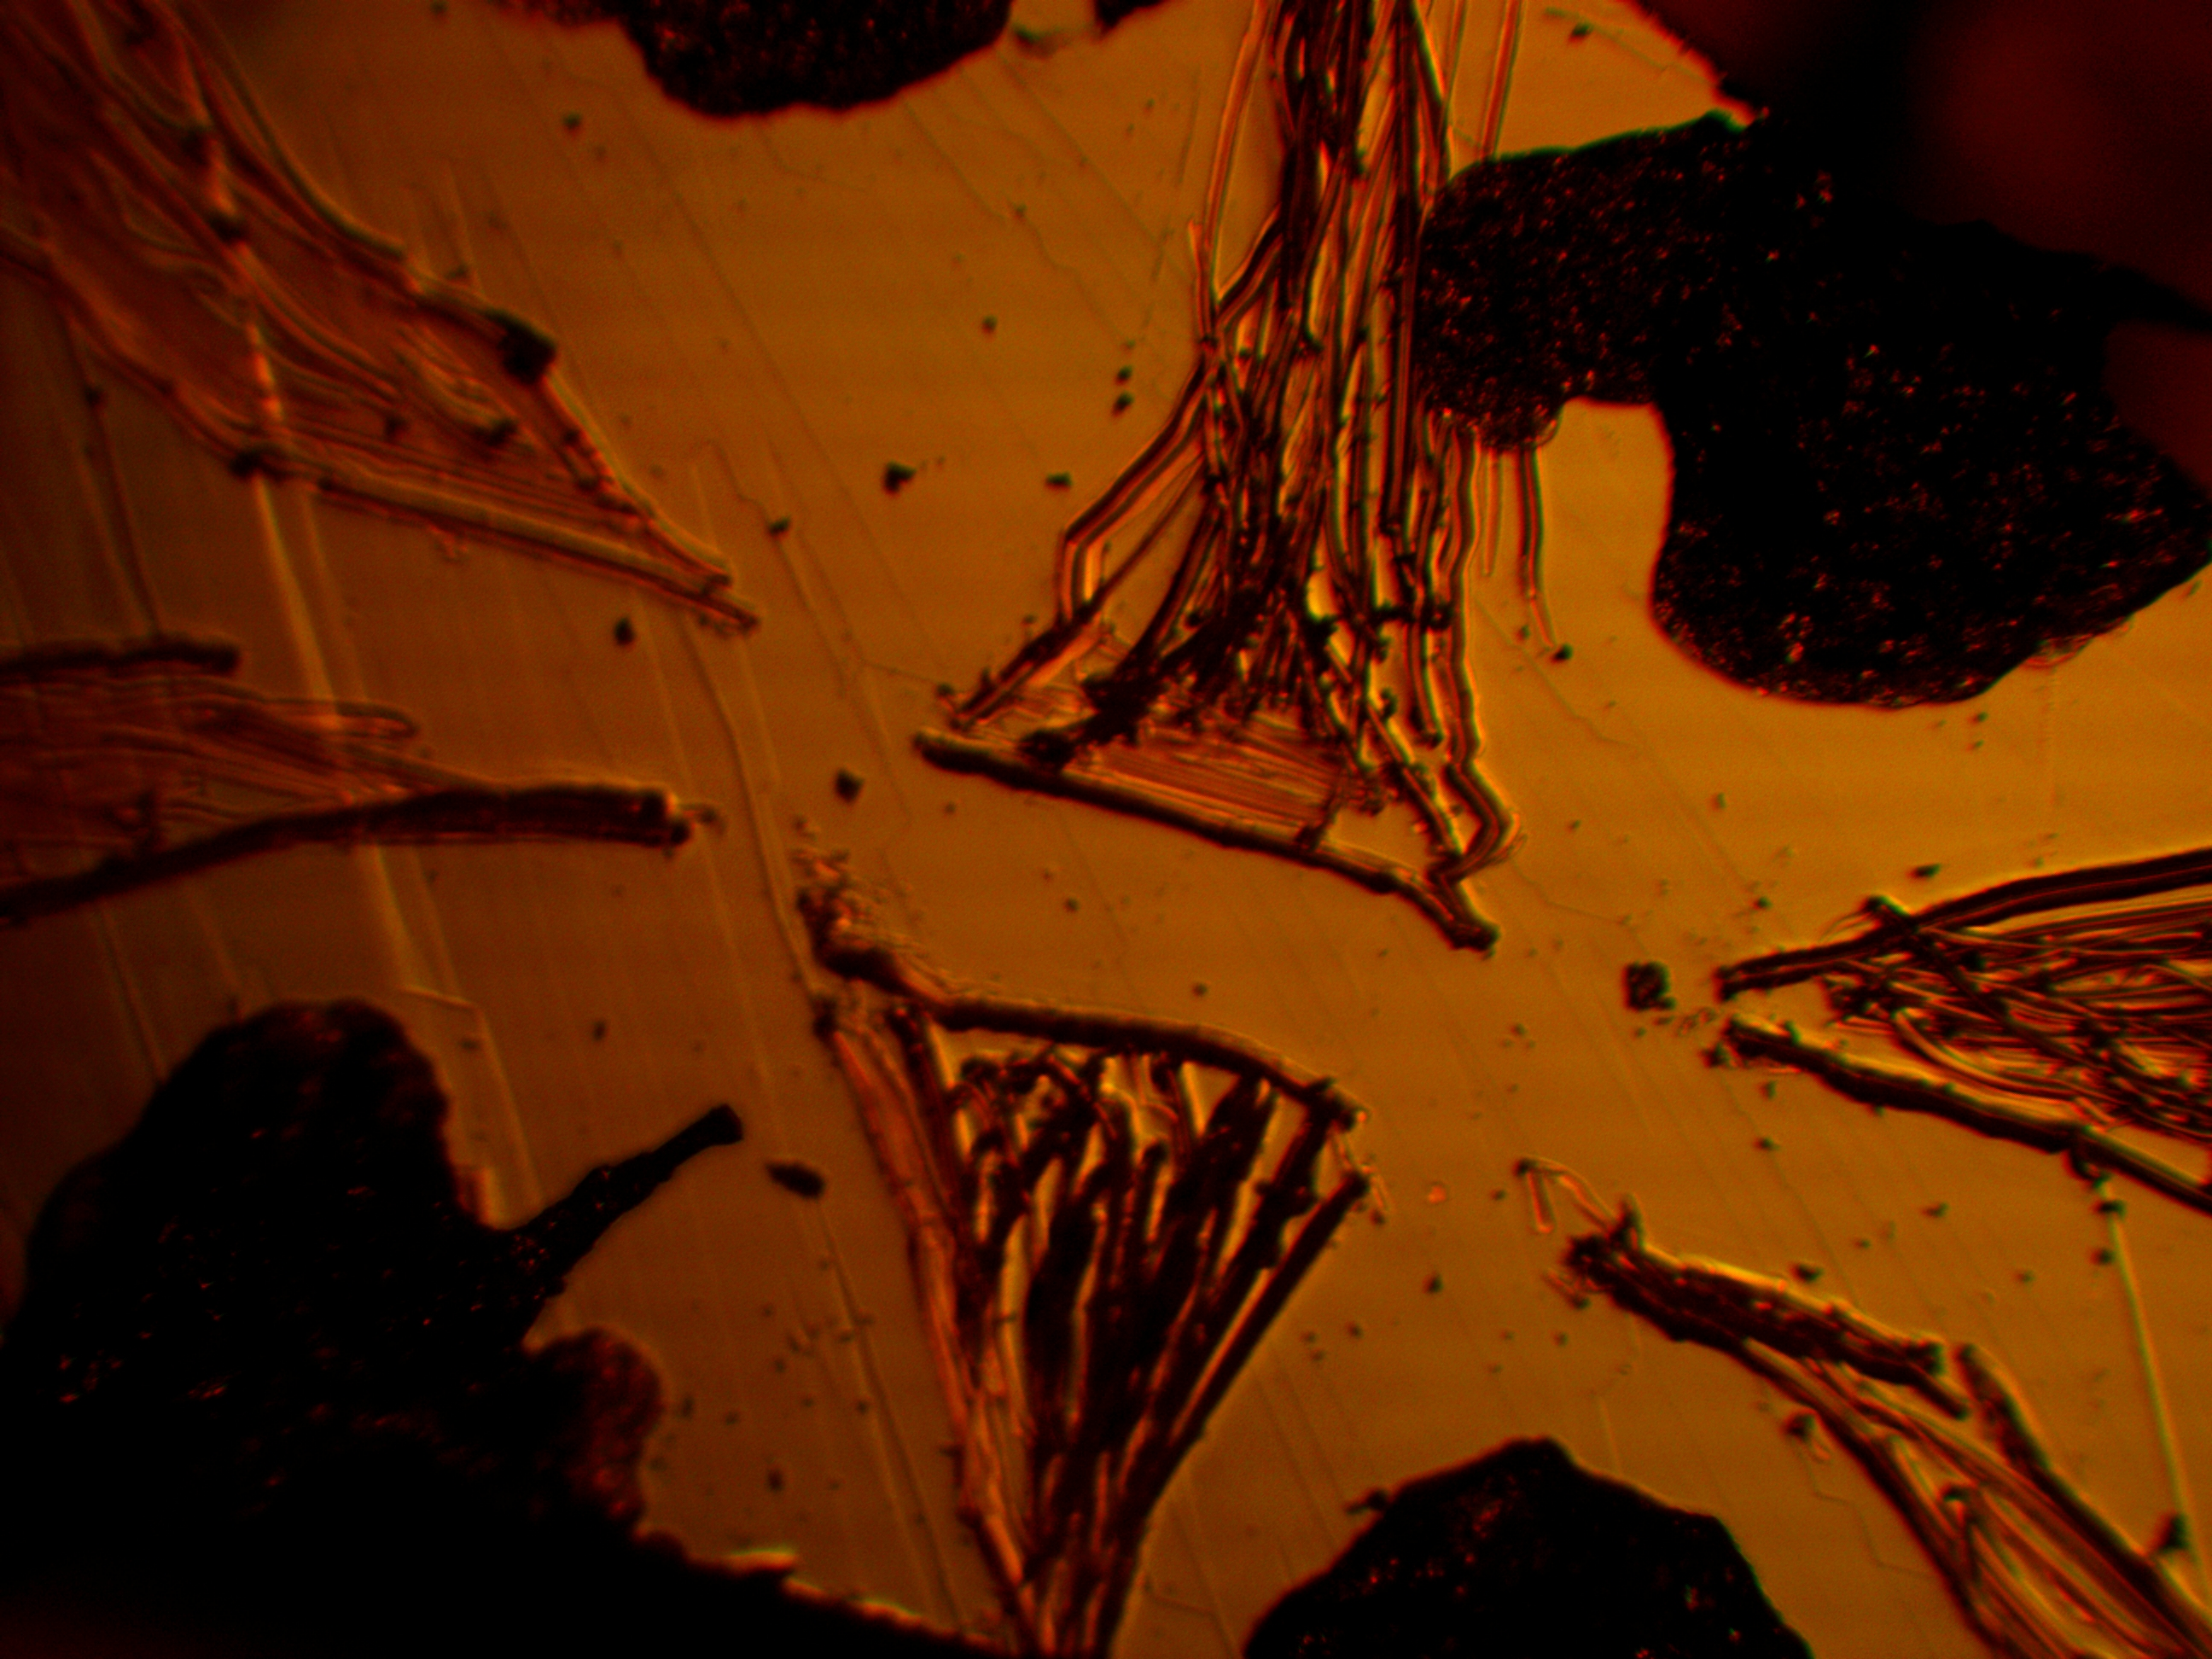
\includegraphics[width=0.5\linewidth]{746.jpg}
\end{center}
\caption{fig1. 746 $Bi_2Se_3$ sample  }
\label{fig:fig1}
\end{figure}
In the fig1. the photo of sample and contacts is presented. Current is aplied to contuct  6 and 3 via resistor 10M Ohm, the lockin voltage is 5V. We measure Rxx between contucts  1 and 2, Rxy  between  2 and 4. 
\newline
Geometrical parametr $\frac{S}{l}=0.2518\pm0.0004$
\newline
Current $R_{xx}$ N6 and N 3
\newline
Potential $R_{xx}$ N1 and N 2
\newline
Potential $R_{xy}$ N2 and N 4
\newline

\begin{table}[H]
\begin{tabular}{l l l l l l l}
\toprule
\textbf{•} & \textbf{1} & \textbf{2} & \textbf{3}& \textbf{4}& \textbf{5}& \textbf{6}\\
\toprule
 1&   & 6K Ohm & 17K Ohm & 11,2K Ohm &  & 6K Ohm\\
 2 & 6,4K Ohm &  &14,4K Ohm & 8,4K Ohm &  &8,5K Ohm\\
 3 & 10,6K Ohm & 14,3K Ohm & & 19,8K Ohm &  & 18,8K Ohm\\
 4 & 11,3K Ohm & 8,4K Ohm &19,8K Ohm &  &  & 13,6K Ohm\\
 5 &  &  &  &  &  \\
 6 & 6K Ohm & 8,5K Ohm &18,8K Ohm &13,6K Ohm &  &\\
\bottomrule
\end{tabular}
\caption{Bi2Se3 (746) R b-w contacts}
\label{tab:Bi2Se3 (746) R b-w contacts}
\end{table}
The resistance of between N5 and N-, $R_5>100K Ohm$, but it is not a problem(3 potential contacts is acceptable for transport measurements).
%-----------------------------------------
\experiment{Measurements}
The sample is putted into Cryogenic Transport Measurement System(CFMS) and field dependancies of Rxx and Rxy are measured with different temperatures(2,4,8,16,32).
List of measurements is dipslayed in  table2.
 \begin{table}[H]
\begin{tabular}{l l l l l}
\toprule
\textbf{File} & \textbf{Field} & \textbf{Temperature}& \textbf{Voltage}& \textbf{Comment}\\
\toprule
Field.sweep.4.lock.in$15.03.18 10.35.51 $& 0T  & from 120K to 5K & 0.1V& Low I\\
Field.sweep.4.lock.in$15.03.18  11.18.22$& 0T  & from 5 to 1.7K&& 0.1V Low I\\
Field.sweep.4.lock.in$15.03.18  11.37.50$& 0T  & from 5.7K to 1.7K & 0.05V&Low I\\
Field.sweep.4.lock.in$15.03.18  12.00.15$& from 1T to 1T  & 2K & 0.1V & Low I\\
Field.sweep.4.lock.in$15.03.18  12.16.32$& from 1T to -1T  & 2K & 0.1V& Low I\\
Field.sweep.4.lock.in$15.03.18  13.08.18$& from 1T to -1T  & 2K & 5V& Ok\\
Field.sweep.4.lock.in$15.03.18  14.44.10$& from -1T to 1T  & 2K &5V & Ok\\
Field.sweep.4.lock.in$15.03.18  14.55.26$& from 4T to -4T  & 2K &5V & Ok\\
Field.sweep.4.lock.in$15.03.18  15.26.28$& from -4T to 4T  & 4K &5V & noisy\\
Field.sweep.4.lock.in$15.03.18  16.06.11$& from -4T to 4T  & 8K &5V & Ok\\
Field.sweep.4.lock.in$15.03.18  16.38.40$& from 4T to -4T  & 16K &5V & Ok\\
Field.sweep.4.lock.in$15.03.18  17.26.48$& from 4T to -4T  & 32K &5V & Ok\\
Field.sweep.4.lock.in$15.03.18  18.29.31$& from 0T to 14T  & 2K &5V & Ok\\
Field.sweep.4.lock.in$15.03.18  19.42.59$& from 4T to -4T  & 4K &5V & Ok\\


\bottomrule
\end{tabular}
\caption{Measurements and files}
\label{tab:Measurements and files}
\end{table}
%-----------------------------------------
\experiment{Results}
In order to find out charge mobility and consentration we analize transport measurements.
For each temperature we have field dependance from -4T to 4T(2,4,8,16,32). After symmetrization we get $R_H$, n and $ \mu$
\newline
RRR=1.43
\newline
\normalsize \textbf{2Kelv}\\
\begin{figure}[H] % Example of including images
\begin{center}
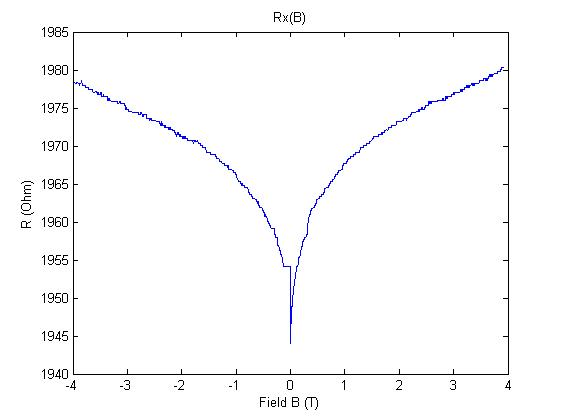
\includegraphics[width=1\linewidth]{7462kRx(B).jpg}
\end{center}
\caption{2Kelvins Rx(B)}
\label{fig:fig2}
\end{figure}

\begin{figure}[H] % Example of including images
\begin{center}
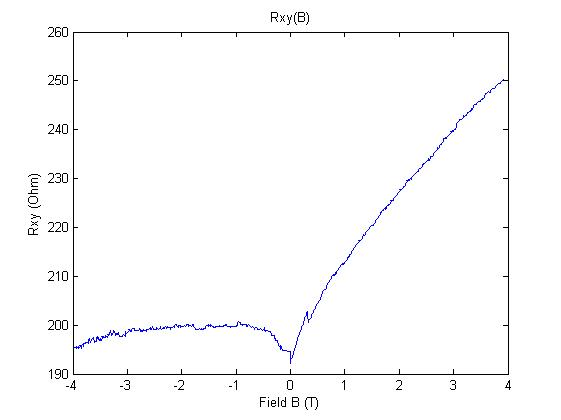
\includegraphics[width=1\linewidth]{7462kRy(B).jpg}
\end{center}
\caption{2Kelvins Ry(B)}
\label{fig:fig3}
\end{figure}

\begin{figure}[H] % Example of including images
\begin{center}
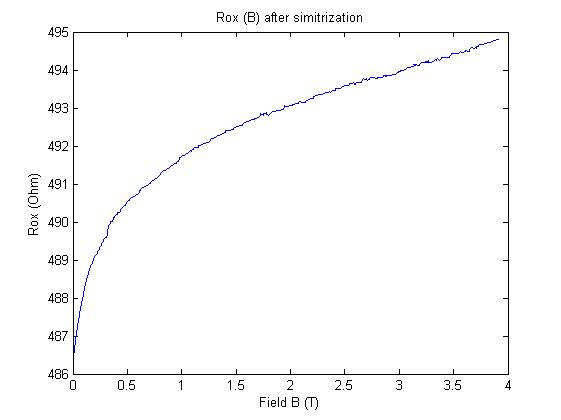
\includegraphics[width=1\linewidth]{7462kRox.jpg}
\end{center}
\caption{2Kelvins Rx(B)  after symetrization} 
\label{fig:fig4}
\end{figure}


\begin{figure}[H] % Example of including images
\begin{center}
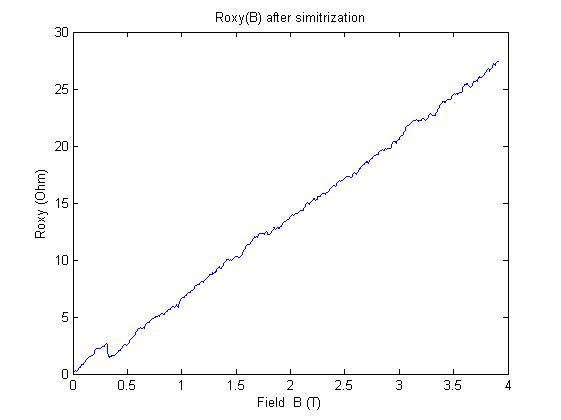
\includegraphics[width=1\linewidth]{7462kRoy.jpg}
\end{center}
\caption{2Kelvins Ry(B)  after symetrization} 
\label{fig:fig5}
\end{figure}



\normalsize \textbf{2Kelv}\\
$R_H=7.011 \frac{Ohm}{T}$
\newline
$n=8.9*10^{13} cm^{-2}$
\newline
$\mu=0.0142 \frac{m^2}{V*s}$
\newline
\newline
\normalsize \textbf{4Kelv}\\
\begin{figure}[H] % Example of including images
\begin{center}
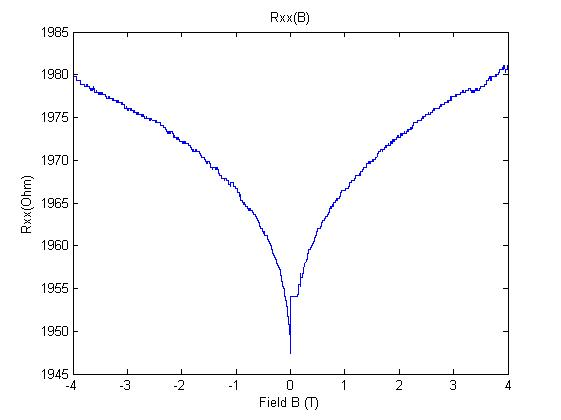
\includegraphics[width=1\linewidth]{7464kRx(B).jpg}
\end{center}
\caption{4Kelvins Rx(B)}
\label{fig:fig6}
\end{figure}

\begin{figure}[H] % Example of including images
\begin{center}
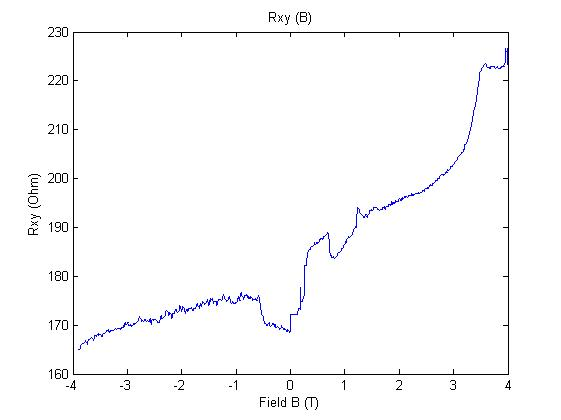
\includegraphics[width=1\linewidth]{7464kRy(B).jpg}
\end{center}
\caption{4Kelvins Ry(B)}
\label{fig:fig7}
\end{figure}

\begin{figure}[H] % Example of including images
\begin{center}
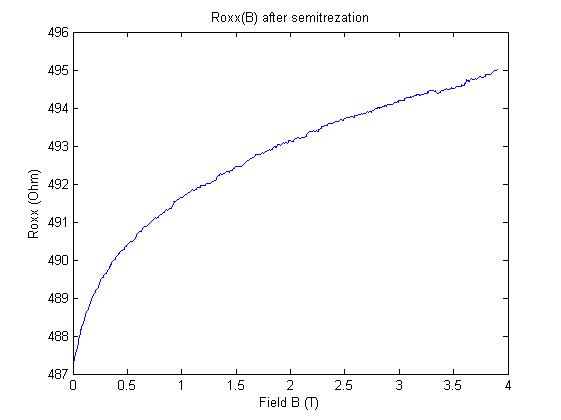
\includegraphics[width=1\linewidth]{7464kRoxx.jpg}
\end{center}
\caption{4Kelvins Rx(B)  after symetrization} 
\label{fig:fig8}
\end{figure}


\begin{figure}[H] % Example of including images
\begin{center}
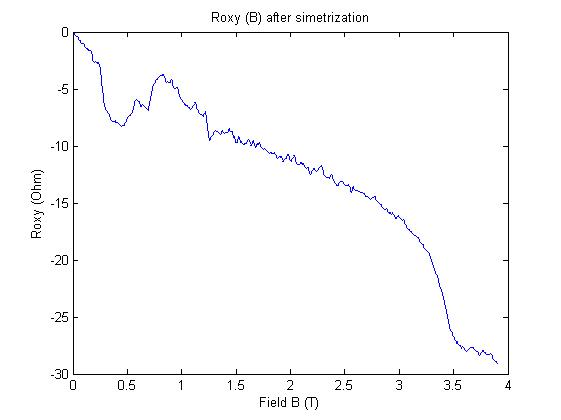
\includegraphics[width=1\linewidth]{7464kRoxy.jpg}
\end{center}
\caption{4Kelvins Ry(B)  after symetrization} 
\label{fig:fig9}
\end{figure}

\normalsize \textbf{4Kelv}\\
$R_H=6.123 \frac{Ohm}{T}$
\newline
$n=1.02*10^{14} cm^{-2}$
\newline
$\mu=0.0123 \frac{m^2}{V*s}$
\newline
\newline


\normalsize \textbf{8Kelv}\\
\begin{figure}[H] % Example of including images
\begin{center}
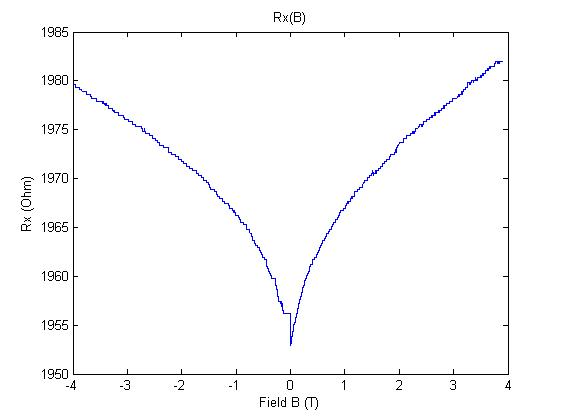
\includegraphics[width=1\linewidth]{7468kRx(B).jpg}
\end{center}
\caption{8Kelvins Rx(B)}
\label{fig:fig10}
\end{figure}

\begin{figure}[H] % Example of including images
\begin{center}
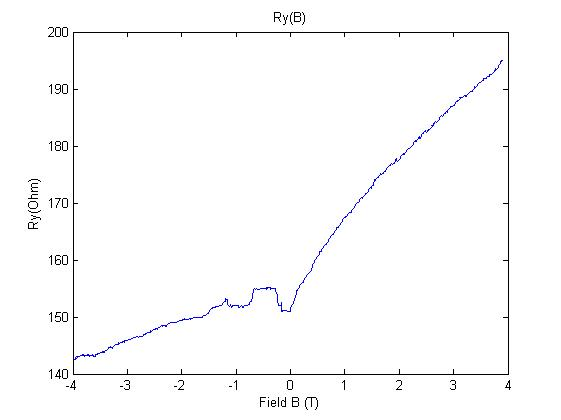
\includegraphics[width=1\linewidth]{7468kRy(B).jpg}
\end{center}
\caption{8Kelvins Ry(B)}
\label{fig:fig11}
\end{figure}

\begin{figure}[H] % Example of including images
\begin{center}
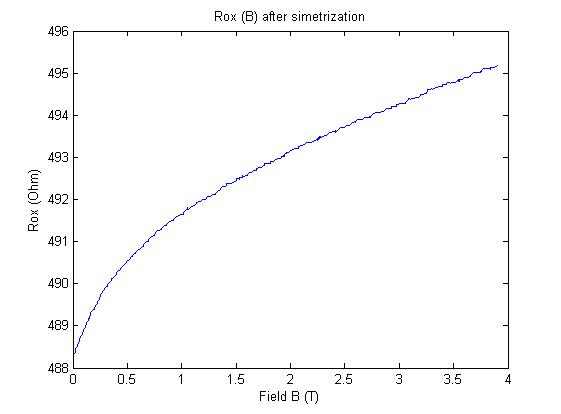
\includegraphics[width=1\linewidth]{7468kRox.jpg}
\end{center}
\caption{8Kelvins Rx(B)  after symetrization} 
\label{fig:fig12}
\end{figure}


\begin{figure}[H] % Example of including images
\begin{center}
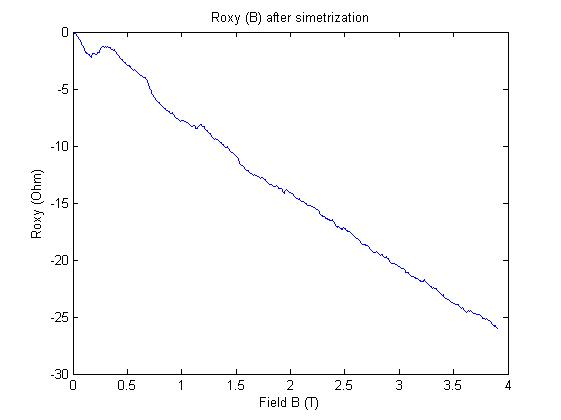
\includegraphics[width=1\linewidth]{7468kRoxy.jpg}
\end{center}
\caption{8Kelvins Ry(B)  after symetrization} 
\label{fig:fig13}
\end{figure}

\normalsize \textbf{8Kelv}\\
$R_H=6.7049 \frac{Ohm}{T}$
\newline
$n=9.3*10^{13} cm^{-2}$
\newline
$\mu=0.0135 \frac{m^2}{V*s}$
\newline
\newline
\newline
\normalsize \textbf{16Kelv}\\
\begin{figure}[H] % Example of including images
\begin{center}
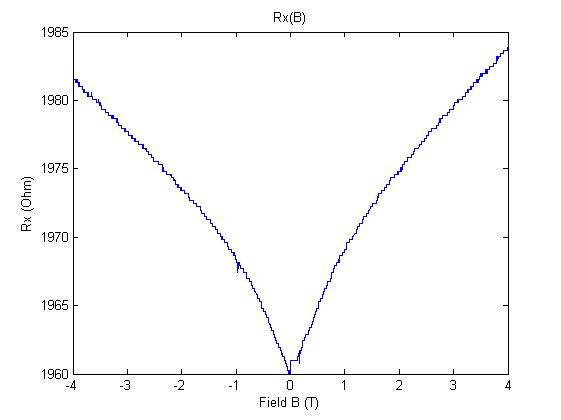
\includegraphics[width=1\linewidth]{74616kRx(B).jpg}
\end{center}
\caption{16Kelvins Rx(B)}
\label{fig:fig14}
\end{figure}


\begin{figure}[H] % Example of including images
\begin{center}
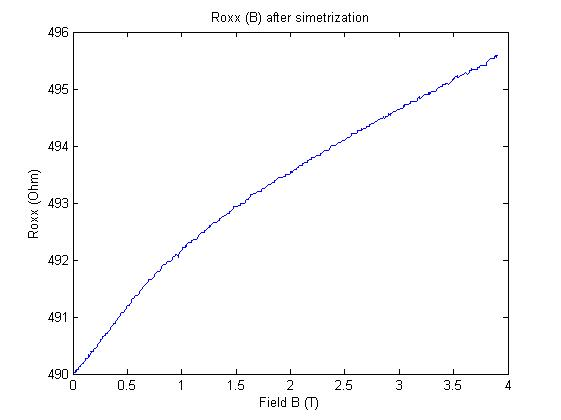
\includegraphics[width=1\linewidth]{74616kRox.jpg}
\end{center}
\caption{16Kelvins Rx(B)  after symetrization} 
\label{fig:fig16}
\end{figure}


\begin{figure}[H] % Example of including images
\begin{center}
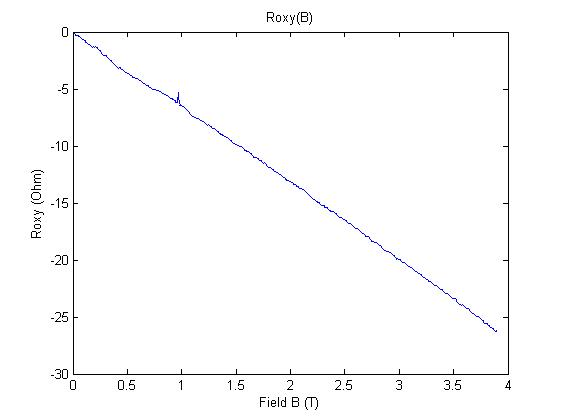
\includegraphics[width=1\linewidth]{74616kRoxy.jpg}
\end{center}
\caption{16Kelvins Ry(B)  after symetrization} 
\label{fig:fig17}
\end{figure}
\normalsize \textbf{16Kelv}\\
$R_H=6.6175 \frac{Ohm}{T}$
\newline
$n=9.36*10^{13} cm^{-2}$
\newline
$\mu=0.0135 \frac{m^2}{V*s}$
\newline
\newline
\newline
\normalsize \textbf{32Kelv}\\
\begin{figure}[H] % Example of including images
\begin{center}
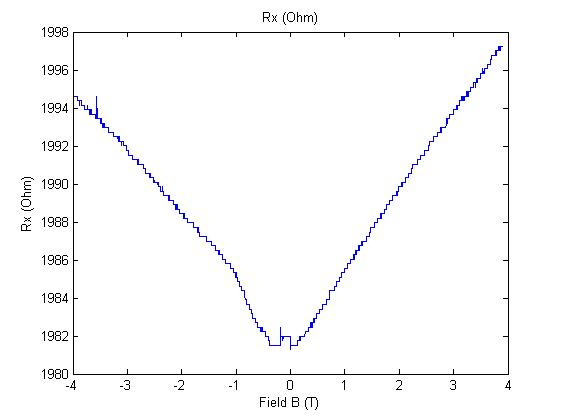
\includegraphics[width=1\linewidth]{74632kRx(B).jpg}
\end{center}
\caption{32Kelvins Rx(B)}
\label{fig:fig10}
\end{figure}

\begin{figure}[H] % Example of including images
\begin{center}
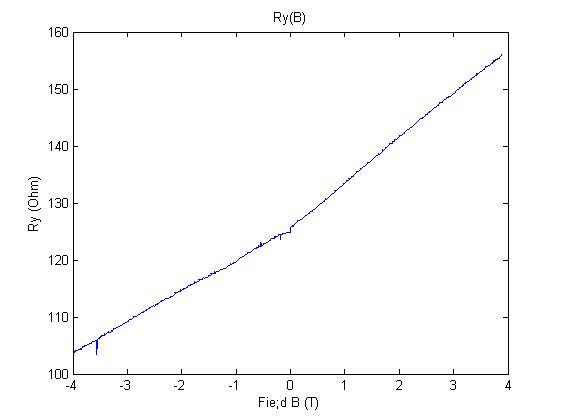
\includegraphics[width=1\linewidth]{74632kRy(B).jpg}
\end{center}
\caption{32Kelvins Ry(B)}
\label{fig:fig11}
\end{figure}

\begin{figure}[H] % Example of including images
\begin{center}
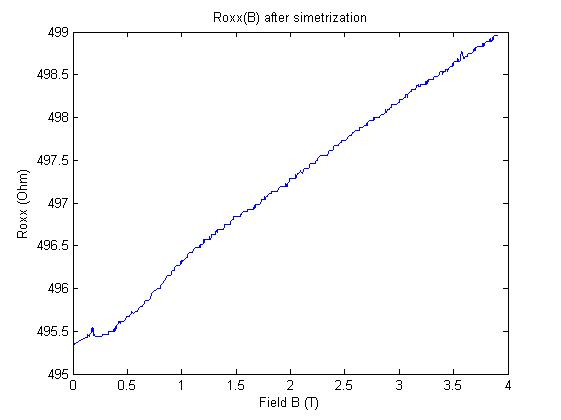
\includegraphics[width=1\linewidth]{74632kRox.jpg}
\end{center}
\caption{32Kelvins Rx(B)  after symetrization} 
\label{fig:fig12}
\end{figure}


\begin{figure}[H] % Example of including images
\begin{center}
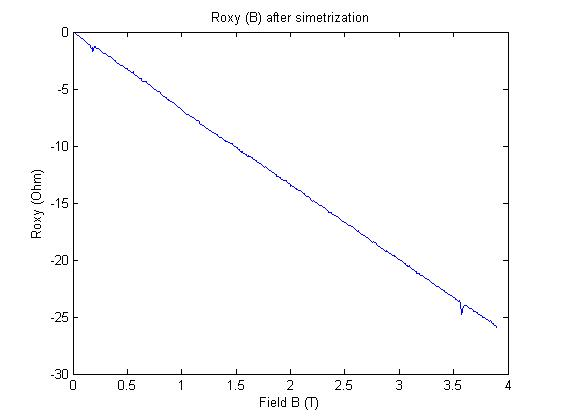
\includegraphics[width=1\linewidth]{74632kRoxy.jpg}
\end{center}
\caption{32Kelvins Ry(B)  after symetrization} 
\label{fig:fig13}
\end{figure}
\normalsize \textbf{32Kelv}\\
$R_H=6.6373 \frac{Ohm}{T}$
\newline
$n=9.41*10^{13} cm^{-2}$
\newline
$\mu=0.0133 \frac{m^2}{V*s}$
\newline



\labday{ 26, 28 March 2018, Transport measurements 747 $Bi_2Se_3$ doped with Sr}
\experiment{Sample 747}
Resistor $=$1M Ohm
Voltage 1V
8-11 current
10-12 rx
10-7 ry \newline
The sample is putted into Cryogenic Transport Measurement System(CFMS) and field dependancies of Rxx and Rxy are measured with  temperature 2,4,8,16,32Kelv.
In the fig1. and fig2. the  photo and scheme of sample contacts is presented. Current is aplied to contact  1 and 4 via resistor 1MOhm, the lockin voltage is 1V. We measure Rxx between contacts  2 and 3, Rxy  between  2 and 6. 
\newline
\begin{figure}[H] % Example of including images
\begin{center}
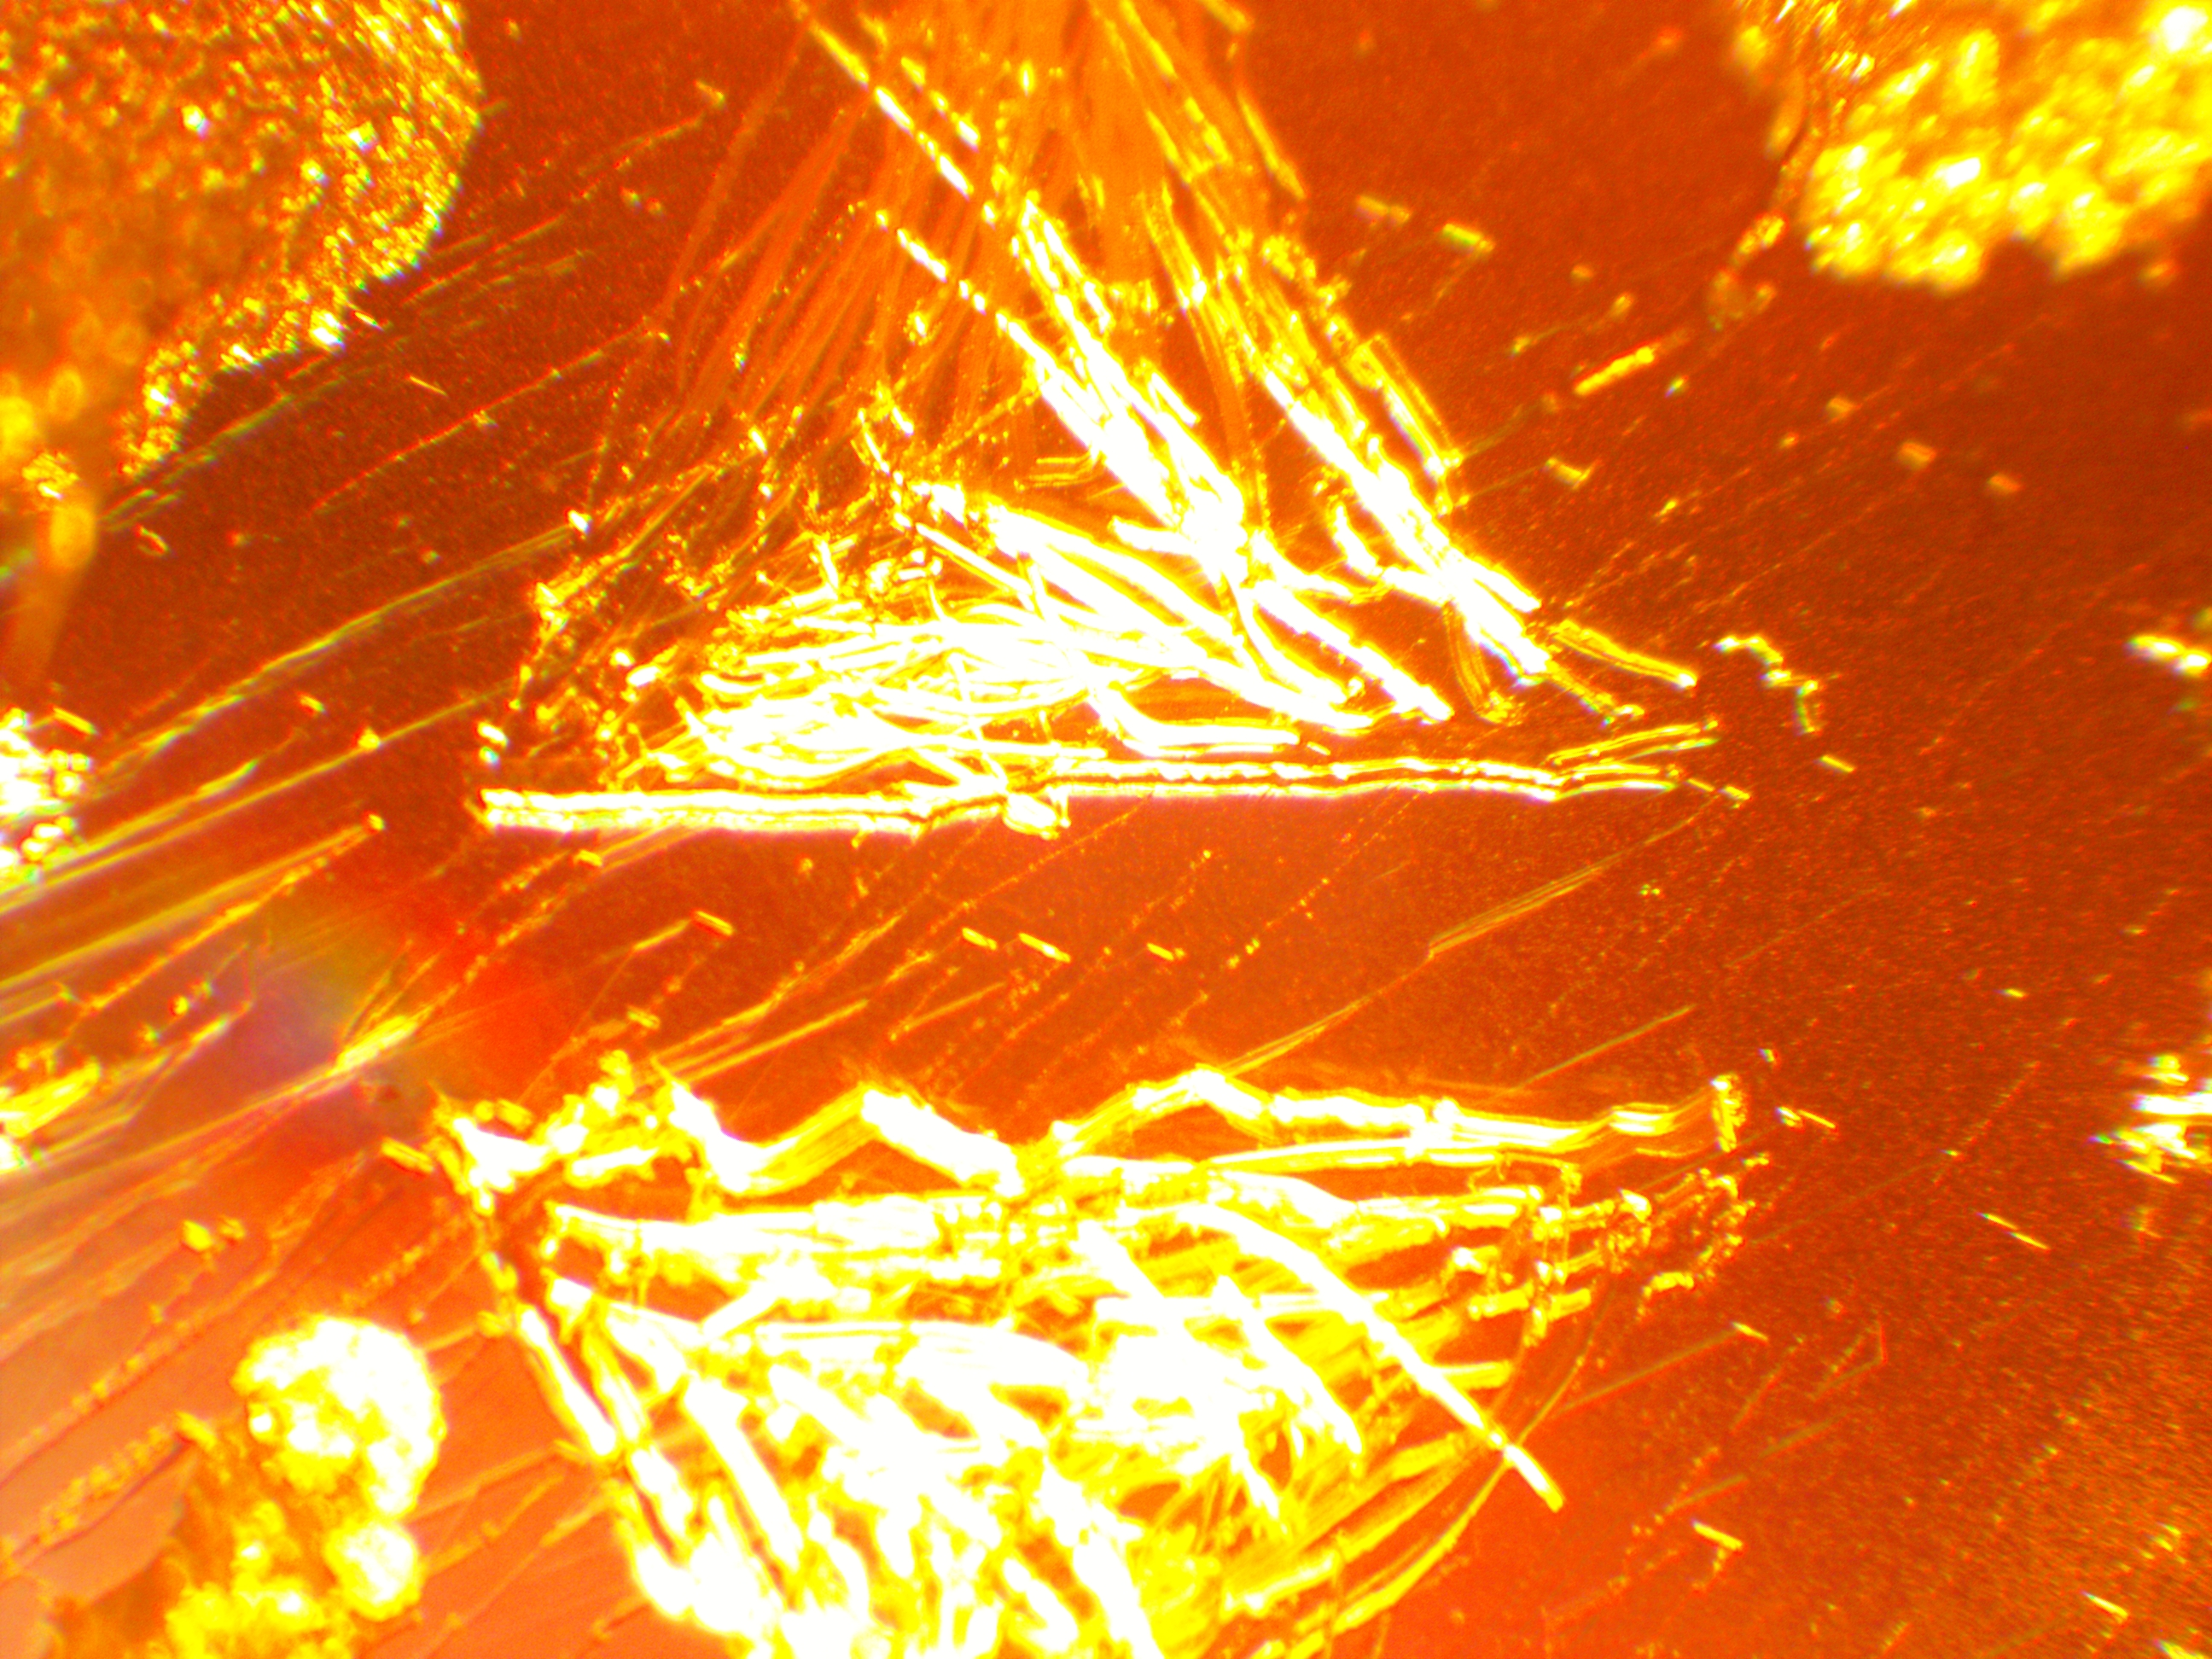
\includegraphics[width=0.5\linewidth]{747.jpg}
\end{center}
\caption{fig1. 747 $Bi_2Se_3$ sample  }
\label{fig:fig1}
\end{figure}
\begin{figure}[H] % Example of including images
\begin{center}
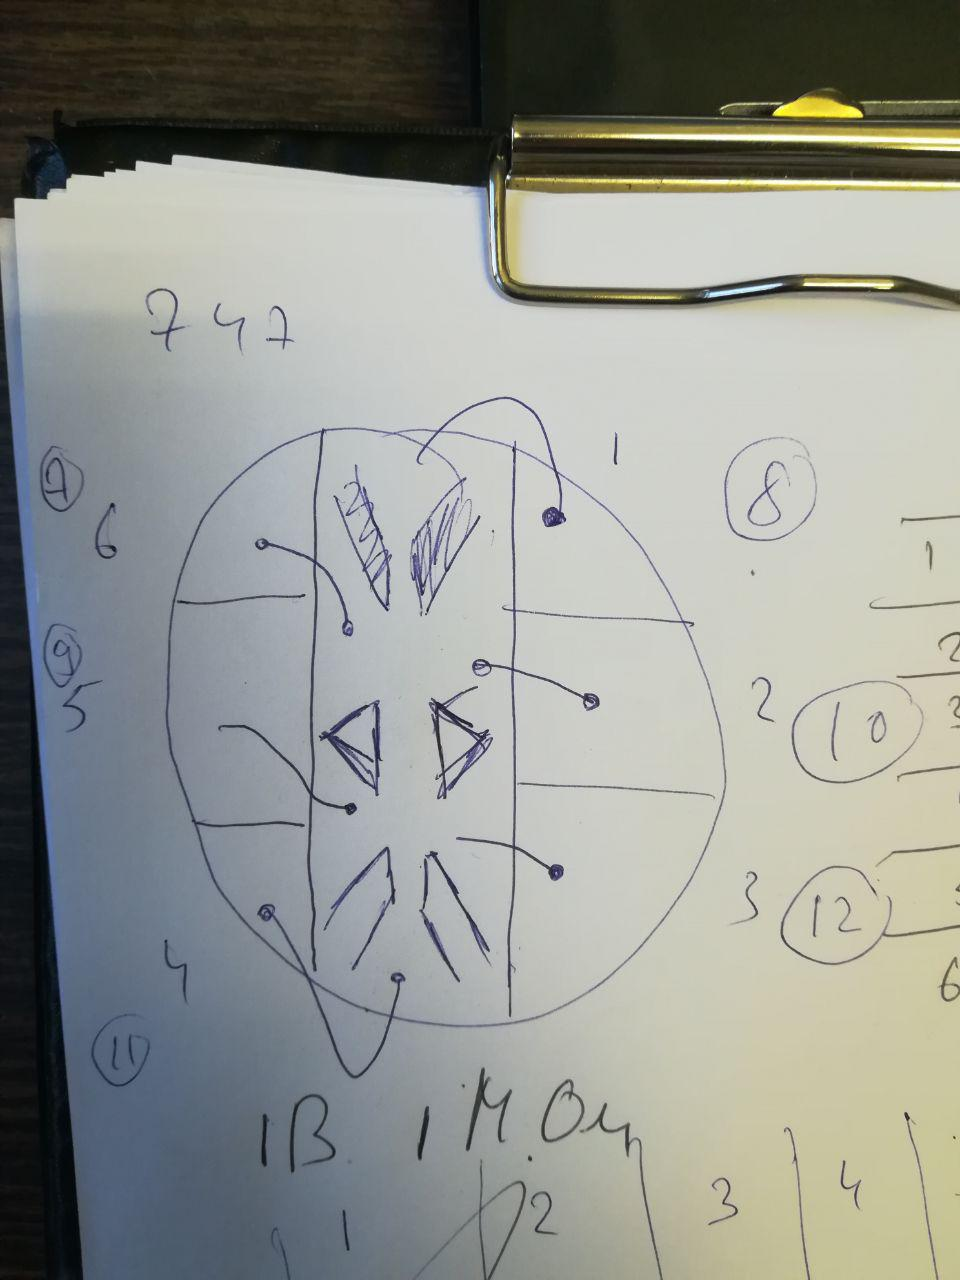
\includegraphics[width=0.5\linewidth]{747schematic.jpg}
\end{center}
\caption{fig2. 746 $Bi_2Se_3$ sample schema  }
\label{fig:fig1}
\end{figure}
Geometrical parametr $\frac{S}{l}=0.1759\pm0.014$
\newline
\begin{table}[H]
\begin{tabular}{l l l l l l l}
\toprule
\textbf{•} & \textbf{1} & \textbf{2} & \textbf{3}& \textbf{4}& \textbf{5}& \textbf{6}\\
\toprule
 1&   & 21K Ohm & 22.2K Ohm & 20,7K Ohm & 8.4K Ohm & 8.1K Ohm\\
 2 & 21.9K Ohm &  &7.9K Ohm & 6.3K Ohm & 21.8K Ohm &23.2K Ohm\\
 3 & 22.7K Ohm & 8.0K Ohm & & 3.9K Ohm & 22.4K Ohm & 24.7K Ohm\\
 4 & 21,1K Ohm & 6.5K Ohm &3.9K Ohm &  & 20.9Kohm & 22,3K Ohm\\
 5 &8.6K Ohm  & 21.6K Ohm &21.3K Ohm  &20.3Kohm & &6.5K Ohm  \\
 6 & 6.5K Ohm & 23,5K Ohm &23,9K Ohm &22,4K Ohm &10.6K Ohm  &\\
\bottomrule
\end{tabular}
\caption{Bi2Se3 (747) R b-w contacts}
\label{tab:Bi2Se3 (747) R b-w contacts}
\end{table}

%-----------------------------------------
\experiment{Measurements}
List of measurements is dipslayed in  table1.
 \begin{table}[H]
\begin{tabular}{l l l l l}
\toprule
\textbf{File} & \textbf{Field} & \textbf{Temperature}& \textbf{Voltage}& \textbf{Comment}\\
\toprule
Field.sweep.4.lock.in$26.03.18 19.27.29$& 0T  & from 240K to 2K & 1V& OK\\
Field.sweep.4.lock.in$26.03.18 20.16.18$& form -6T to 6T  & 2K & 1V& OK\\
Field.sweep.4.lock.in$26.03.18 20.54.04$& form 3T to -0.5  & 2K & 1V& Com1\\
Field.sweep.4.lock.in$28.03.18 18.26.15$& 0T  & from 290K to 2K & 1V& Com1\\
Field.sweep.4.lock.in$28.03.18 19.51.28$& from 2 to -2  &  2K & 1V&Step=0.2T\\
Field.sweep.4.lock.in$28.03.18 20.15.04$& from -2 to 2  &  2K & 1V&Step=0.2T\\
Field.sweep.4.lock.in$28.03.18 $& from 14 to -14  &  2K & 1V&Step=0.4T\\
Field.sweep.4.lock.in$28.03.18 20.48.24$& from -2 to 2  &  4K & 1V&Step=0.2T\\
Field.sweep.4.lock.in$28.03.18 21.09.32$& from 2 to -2  &  8K & 1V&Step=0.2T\\
Field.sweep.4.lock.in$28.03.18 21.51.44$& from -1.5 to 1.5  &  16K & 1V&Step=0.2T\\
Field.sweep.4.lock.in$28.03.18 22.15.44$& from 1.5 to -1.5  &  32K & 1V&Step=0.2T\\


\bottomrule
\end{tabular}
\caption{Measurements and files}
\label{tab:Measurements and files}
\end{table}
COM1: I have changed
Rx= 10-12
Ry=9-12
\experiment{Results}
RRR=1.5

 \labday{ 31 March 2018, Weak antilocalisation 746 $Bi_2Se_3$ doped with Sr}
\experiment{Theory}
\experiment{Measurements}
We had problems with switching in the magnit cercuit, accoding to fix it the field step is decreased to 0.1T per minute.
The circuit conditions are the saim as was in previous experiment.(R=1MOhm, V=1Volt)
List of measurements is dipslayed in  table1.
 \begin{table}[H]
\begin{tabular}{l l l l l}
\toprule
\textbf{File} & \textbf{Field} & \textbf{Temperature}& \textbf{Voltage}& \textbf{Comment}\\
\toprule
Field.sweep.4.lock.in$31.03.18 14.07.07$& from 2 to -2  & 2K & 1V& 0.2T/min\\
Field.sweep.4.lock.in$31.03.18 14.29.00$& from -2 to 2  & 4K & 1V& 0.2T/min\\
Field.sweep.4.lock.in$31.03.18 15.06.18$& from 2 to -2  & 8K & 1V& 0.2T/min\\
Field.sweep.4.lock.in$31.03.18 15.26.37$& from -2 to 2  & 16K & 1V& 0.2T/min\\
Field.sweep.4.lock.in$31.03.18 16,04,07$& from 2 to -2  & 32K& 1V& 0.2T/min\\
\bottomrule
\end{tabular}
\caption{Measurements and files}
\label{tab:Measurements and files}
\end{table}
In order to understand how magnitoresistivity depends on temperature next measurements have been done:
\begin{table}[H]
\begin{tabular}{l l l l l}
\toprule
\textbf{File} & \textbf{Field} & \textbf{Temperature}& \textbf{Voltage}& \textbf{Comment}\\
\toprule

Field.sweep.4.lock.in$31.03.18 16.35.48$& from -6 to 6  & 32K & 1V& 0.5T/min\\
Field.sweep.4.lock.in$31.03.18 17.20.22$& from 6 to -6  & 16K & 1V& 0.5T/min\\
Field.sweep.4.lock.in$31.03.18 17.56.52$& from -6 to 6  & 8K & 1V& 0.5T/min\\
Field.sweep.4.lock.in$31.03.18 18.30.56$& from 6 to -6  & 4K& 1V& 0.5T/min\\
Field.sweep.4.lock.in$31.03.18 19.09.26$& from -6 to 6  & 2K& 1V& 0.5T/min\\
\bottomrule
\end{tabular}
\caption{Measurements and files}
\label{tab:Measurements and files}
\end{table}
\experiment{Results}
2Kelv
\begin{table}[H]
\begin{tabular}{l l l l l}
\toprule
\textbf{Temperature} & \textbf{$\alpha$} & \textbf{$l_{\varphi}*10^{-7}$m}\\
\toprule
2&  0.549 & 1.876 \\
4&  0.555 & 1.366 \\
8&  0.659 & 0.813 \\
16& 0.795 & 0.477 \\
16& 0.647 & 0.329 \\

\bottomrule
\end{tabular}
\caption{WAL Results}
\label{tab:WAL Results}
\end{table}
\labday{ ??? 2018, Transport mesuarments SOT 400}
\experiment{SOT 400 sample}
Sample from Ole. Photo
\newline
Geometrical parametr $\frac{S}{l}=0.\pm0.0$
\newline
\begin{table}[H]
\begin{tabular}{l l l l l l l}
\toprule
\textbf{•} & \textbf{1} & \textbf{2} & \textbf{3}& \textbf{4}& \textbf{5}& \textbf{6}\\
\toprule
 1&   & 1.21K Ohm & 33.6K Ohm & 2.14K Ohm & 1.63K Ohm & 1.96K Ohm\\
 2 & 1.21K Ohm &  & 35.0K Ohm & 1.9K Ohm & 1.4K Ohm &1.7K Ohm\\
 3 & 15.6K Ohm & 10.8K Ohm & & 15.8K Ohm & 30.3K Ohm & 10.2K Ohm\\
 4 & 3.5K Ohm & 2.5K Ohm &32K Ohm &  & 1.5K Ohm & 1.8K Ohm\\
 5 &1.6K Ohm  & 1.4K Ohm &54.0K Ohm  &1.4K Ohm & &1.2K Ohm  \\
 6 & 1.8K Ohm & 1.6K Ohm &102K Ohm &1.8K Ohm &1.2K Ohm  &\\
\bottomrule
\end{tabular}
\caption{SOT400 R b-w contacts}
\label{tab:SOT 400 R b-w contacts}
\end{table}

\experiment{SOT 400 measurements}


\labday{ 3 April 2018, Transport measurements 757A $Bi_2Se_3$ doped with Sr}
\experiment{Sample 757}
Geometrical parametr $\frac{S}{l}=0.176$
\newline
\experiment{Measurements}
List of measurements is dipslayed in  table1.
 \begin{table}[H]
\begin{tabular}{l l l l l}
\toprule
\textbf{File} & \textbf{Field} & \textbf{Temperature}& \textbf{Voltage}& \textbf{Comment}\\
\toprule
Field.sweep.4.lock.in$03.04.18 21.58.20$& from 10T to 0T   & 2K & 1V& 0.5T/min\\
Field.sweep.4.lock.in$03.04.18 23.45.47$& from 6 to -6T   & 2K & 1V& 0.5T/min\\
Field.sweep.4.lock.in$04.04.18 $& from -6 to 6T   & 2K & 1V& 0.5T/min\\
Field.sweep.4.lock.in$04.04.18 00.51.20$& from -6 to 6T   & 2K & 1V& 0.5T/min\\
Field.sweep.4.lock.in$04.04.18 01.32.27$& from 2T to -2T   & 2K & 1V& 0.2T/min\\
Field.sweep.4.lock.in$04.04.18 02.36.54$& from -6T to 6T   & 4K & 1V& 0.5T/min\\
Field.sweep.4.lock.in$04.04.18 03.07.07$& from 6T to 0T   & 4K & 1V& 0.5T/min\\
Field.sweep.4.lock.in$04.04.18 02.03.54$& from 2T to -2T   & 4K & 1V& 0.2T/min\\
Field.sweep.4.lock.in$04.04.18 03.38.07$& from -6T to 6T   & 8K & 1V& 0.5T/min\\
Field.sweep.4.lock.in$04.04.18 04.22.10$& from 2T to -2T   & 8K & 1V& 0.2T/min\\
Field.sweep.4.lock.in$04.04.18 05.05.47$& from -6T to 6T   & 16K & 1V& 0.5T/min\\
Field.sweep.4.lock.in$04.04.18 $& from 2T to -2T   & 16K & 1V& 0.2T/min\\
Field.sweep.4.lock.in$04.04.18 05.45.38$& from -6T to 6T   & 32K & 1V& 0.5T/min\\
Field.sweep.4.lock.in$04.04.18 $& from 2T to -2T   & 32K & 1V& 0.2T/min\\



\bottomrule
\end{tabular}
\caption{Measurements and files}
\label{tab:Measurements and files}
\end{table}

\experiment{Results}
RRR=1.64
\newline
\normalsize \textbf{2Kelv}\\
$R_H=13.43 \frac{Ohm}{T}$
\newline
$n=4.65*10^{13} cm^{-2}$
\newline
$\mu= 0.0681\frac{m^2}{V*s}$
\newline
\newline

\normalsize \textbf{4Kelv}\\
$R_H=13.42 \frac{Ohm}{T}$
\newline
$n=4.66*10^{13} cm^{-2}$
\newline
$\mu= 0.0682\frac{m^2}{V*s}$
\newline
\newline


\normalsize \textbf{8Kelv}\\
$R_H=13.34 \frac{Ohm}{T}$
\newline
$n=4.69*10^{13} cm^{-2}$
\newline
$\mu= 0.0680\frac{m^2}{V*s}$
\newline
\newline

\normalsize \textbf{16Kelv}\\
$R_H=13.28 \frac{Ohm}{T}$
\newline
$n=4.71*10^{13} cm^{-2}$
\newline
$\mu= 0.0677\frac{m^2}{V*s}$
\newline
\newline

\normalsize \textbf{32Kelv}\\
$R_H=13.27 \frac{Ohm}{T}$
\newline
$n=4.71*10^{13} cm^{-2}$
\newline
$\mu= 0.0673\frac{m^2}{V*s}$
\newline
\newline


%----------------------------------------------------------------------------------------
\labday{ 5 April 2018, Transport measurements 761D $Bi_2Se_3$ covered with Sr}
\experiment{Sample 761D}
Geometrical parametr $\frac{S}{l}=0.336$
\newline
\experiment{Measurements}
List of measurements is dipslayed in  table1.
 \begin{table}[H]
\begin{tabular}{l l l l l}
\toprule
\textbf{File} & \textbf{Field} & \textbf{Temperature}& \textbf{Voltage}& \textbf{Comment}\\
\toprule
Field.sweep.4.lock.in$05.04.18 18.14.47$& 0T   & from 300K to2K & 1V& Ok\\
Field.sweep.4.lock.in$05.04.18 19.49.05$& from 2 T to-2T   & 2K & 1V& 0.2T/min\\
Field.sweep.4.lock.in$05.04.18 20.15.33$& from 2 T to-1.5T   & 2K & 1V& 0.1T/min\\
Field.sweep.4.lock.in$05.04.18 20.51.06$& from -2 T to 2T   & 4K & 1V& 0.2T/min\\
Field.sweep.4.lock.in$05.04.18 $& from 2 T to -2T   & 8K & 1V& 0.2T/min\\
Field.sweep.4.lock.in$05.04.18 $& from -2 T to 2T   & 16K & 1V& 0.2T/min\\
Field.sweep.4.lock.in$05.04.18 $& from -2 T to 2T   & 32K & 1V& 0.2T/min\\




\bottomrule
\end{tabular}
\caption{Measurements and files}
\label{tab:Measurements and files}
\end{table}


\experiment{Results}
RRR=1.22
\newline
\normalsize \textbf{2Kelv}\\
$R_H=11.93 \frac{Ohm}{T}$
\newline
$n=5.23*10^{13} cm^{-2}$
\newline
$\mu= 0.0049\frac{m^2}{V*s}$
\newline
\newline

\normalsize \textbf{4Kelv}\\
$R_H=9.89 \frac{Ohm}{T}$
\newline
$n=6.3*10^{13} cm^{-2}$
\newline
$\mu= 0.0040\frac{m^2}{V*s}$
\newline
\newline


\normalsize \textbf{8Kelv}\\
ABrakadabra Ry(B)=const
\newline
\newline


\normalsize \textbf{16Kelv}\\
ABrakadabra Ry(B)=const
\newline
\newline

\normalsize \textbf{32Kelv}\\
ABrakadabra Ry(B)=const
\newline
\newline


%----------------------------------------------------------------------------------------

%----------------------------------------------------------------------------------------
\labday{ 10 April 2018, Transport measurements 761D $Bi_2Se_3$ after Annealing}
\experiment{Sample 761DAnnealed}
1V frough 1 Mohm l/w=3.1
Problems with temperature
\experiment{Measurements}
List of measurements is dipslayed in  table1.
 \begin{table}[H]
\begin{tabular}{l l l l l}
\toprule
\textbf{File} & \textbf{Field} & \textbf{Temperature}& \textbf{Voltage}& \textbf{Comment}\\
\toprule
Field.sweep.4.lock.in$10.04.18 20.06.51$& 0T   & from 300K to2K & 1V& Ok\\
Field.sweep.4.lock.in$10.04.18 21.34.04$& from -6T to 6T & 2K & 1V& 0.5T/min\\
Field.sweep.4.lock.in$10.04.18 22.07.59$& from 6T to -6T & 4K & 1V& 0.5T/min\\
Field.sweep.4.lock.in$10.04.18 22.34.14$& from 6T to -6T & 4K & 1V& 0.5T/min\\
Field.sweep.4.lock.in$10.04.18 $& from -6T to 6T & 8K & 1V& Errrr\\
Field.sweep.4.lock.in$11.04.18 10.53.50$& from 6T to -6T & 16K & 1V& 0.5T/min\\
Field.sweep.4.lock.in$11.04.18 00_19_39$& from -6T to 6T & 32K & 1V& 0.5T/min\\
Field.sweep.4.lock.in$11.04.18 $& from 2T to -2T & 2K & 1V& Errrr\\
Field.sweep.4.lock.in$11.04.18 $& from -2T to 2T & 4K & 1V& Errrr\\
Field.sweep.4.lock.in$11.04.18 $& from 2T to -2T & 8K & 1V& Errrr\\
Field.sweep.4.lock.in$11.04.18 $& from -2T to 2T & 16K & 1V& Errrr\\
Field.sweep.4.lock.in$10. $& from 2T to -2T & 32K & 1V& Errrr\\
Field.sweep.4.lock.in$10.04.18 $& from -12T to 12T & 32K & 1V& Errrr\\






\bottomrule
\end{tabular}
\caption{Measurements and files}
\label{tab:Measurements and files}
\end{table}


\experiment{Results}
RRR=1.38
\newline
\normalsize \textbf{2Kelv}\\
$R_H=7.81 \frac{Ohm}{T}$
\newline
$n=8*10^{13} cm^{-2}$
\newline
$\mu= 0.0279\frac{m^2}{V*s}$
\newline
\newline

\normalsize \textbf{32Kelv}\\
$R_H=7.76 \frac{Ohm}{T}$
\newline
$n=8,1*10^{13} cm^{-2}$
\newline
$\mu= 0.0293\frac{m^2}{V*s}$
\newline
\newline


%----------------------------------------------------------------------------------------
\labday{ 17 April 2018, Transport measurements 761D $Bi_2Se_3$ after Annealing 300K}
\experiment{Sample 761DAnnealed 300K}
1V frough 1 Mohm l/w=6.1
Problems with temperature
\experiment{Measurements}
List of measurements is dipslayed in  table1.
 \begin{table}[H]
\begin{tabular}{l l l l l}
\toprule
\textbf{File} & \textbf{Field} & \textbf{Temperature}& \textbf{Voltage}& \textbf{Comment}\\
\toprule
Field.sweep.4.lock.in$17.04.18 11.56.39$& 0T   & from 300K to2K & 1V& Ok\\
Field.sweep.4.lock.in$17.04.18 12.53.41$& -2T to 2T   & 32K & 1V& 0.2T/min\\
Field.sweep.4.lock.in$17.04.18 13.29.13$& 2T to -2T   & 16K & 1V& 0.2T/min\\
Field.sweep.4.lock.in$17.04.18 13.58.28$& -2T to 2T   & 8K & 1V& 0.2T/min\\
Field.sweep.4.lock.in$17.04.18 15.00.30$& 2T to -2T   & 4K & 1V& 0.2T/min\\
Field.sweep.4.lock.in$17.04.18 15.33.45$& 2T to -2T   & 2K & 1V& 0.2T/min\\
Field.sweep.4.lock.in$17.04.18 17.23.32$& 6T to -6T   & 32K & 1V& 0.5T/min\\
Field.sweep.4.lock.in$17.04.18 18.30.29$& -6T to 6T   & 2K & 1V& 0.5T/min\\







\bottomrule
\end{tabular}
\caption{Measurements and files}
\label{tab:Measurements and files}
\end{table}


\experiment{Results}
RRR=1.38
\newline

\normalsize \textbf{2Kelv}\\
$R_H=2.88 \frac{Ohm}{T}$
\newline
$n=2.17*10^{14} cm^{-2}$
\newline
$\mu= 0.0082\frac{m^2}{V*s}$
\newline
\newline


\normalsize \textbf{4Kelv}\\
$R_H=2.87 \frac{Ohm}{T}$
\newline
$n=2.18*10^{14} cm^{-2}$
\newline
$\mu= 0.0082\frac{m^2}{V*s}$
\newline
\newline

\normalsize \textbf{8Kelv}\\
$R_H=2.85 \frac{Ohm}{T}$
\newline
$n=2.19*10^{14} cm^{-2}$
\newline
$\mu= 0.0082\frac{m^2}{V*s}$
\newline
\newline


%----------------------------------------------------------------------------------------
\labday{ 21,22 April 2018, Transport measurements 761A and 746A $Bi_2Se_3$}
\experiment{Sample 761A and 746A }
761A l/w=5.7254
\newline
746A  l/w=3.5245
\newline
AUX1 10V -300K 0V --0K
\newline
AUX2 10V 1T   0V 0T
\newline
761A and 746A
\newline
\begin{table}[H]
\begin{tabular}{l l l l l l l}
\toprule
\textbf{•} & \textbf{3} & \textbf{4} & \textbf{5}& \textbf{6}& \textbf{7}& \textbf{9}\\
\toprule
 3&   & 8.9K Ohm & 5.2K Ohm & 6.9K Ohm & 7.1K Ohm & 4.7K Ohm\\
 4 &  &  & 7.1K Ohm & 3.8K Ohm & 3.9K Ohm &6.8K Ohm\\
 5 &  &  & & 5.2K Ohm & 5.3K Ohm & 3.3K Ohm\\
 6 & & & &  & 2.2K Ohm & 4.9K Ohm\\
 7 & & & & & &5.0K Ohm  \\
 9 &  &  & & &  &\\
\bottomrule
\end{tabular}
\caption{761A  R b-w contacts}
\label{tab:761A  R b-w contacts}
\end{table}

\begin{table}[H]
\begin{tabular}{l l l l l l l}
\toprule
\textbf{•} & \textbf{8} & \textbf{10} & \textbf{11}& \textbf{12}& \textbf{13}& \textbf{14}\\
\toprule
 8&   & 14.5K Ohm & 13.7K Ohm & 14.2K Ohm & 14.9K Ohm & 16.5K Ohm\\
 10 &  &  & 8.3K Ohm & 5.5K Ohm & 8.4K Ohm &8.3K Ohm\\
 11 &  &  & & 6.2K Ohm & 7.0K Ohm & 9.1K Ohm\\
 12 & & & &  & 7.0K Ohm & 6.6K Ohm\\
 13 & & & & & &9.2K Ohm  \\
 14 &  &  & & &  &\\
\bottomrule
\end{tabular}
\caption{746A  R b-w contacts}
\label{tab:746A  R b-w contacts}
\end{table}

\experiment{Measurements}
List of measurements is dipslayed in  table1.
 \begin{table}[H]
\begin{tabular}{l l l l l}
\toprule
\textbf{File} & \textbf{Field} & \textbf{Temperature}& \textbf{Voltage}& \textbf{Comment}\\
\toprule
data$21.04.18 13.27.05$& -1T to 1T   & 300K & 1V& 50 Oe/sec\\
data$21.04.18 14.03.17$& 1T to -1T   & 100K & 1V& 50 Oe/sec\\
data$21.04.18 14.19.56$& -1T to 1T   & 77K & 1V& 50 Oe/sec\\
data$21.04.18 14.47.12$& 1T to -1T   & 32K & 1V& 50 Oe/sec\\
data$21.04.18 14.56.128$& -1T to 1T   & 16K & 1V& 50 Oe/sec\\
data$21.04.18 15.12.28$& 1T to -1T   & 8K & 1V& 50 Oe/sec\\
data$21.04.18 15.27.38$& -1T to 1T   & 4K & 1V& 50 Oe/sec\\
data$21.04.18 15.43.51$& 1T to -1T   & 2K & 1V& 50 Oe/sec\\
data$21.04.18 16.19.15$& 0T   & from 2K to 300K & 1V& 50 Oe/sec\\
data$22.04.18 12.39.45$& 0T   & from 300K to 400K & 1V& *\\
data$22.04.18 12.39.45$& -1<->1T  &  400K & 1V& 50 Oe/s multy\\
data$22.04.18 13.58.39$& from -1Tto 1T  &  300K & 1V& 50 50e/s \\
data$22.04.18 15.08.31$& from -1Tto 1T  &  100K & 1V& 50 50e/s \\
data$22.04.18 15.20.12$& from -1Tto 1T  &  77K & 1V& 50 50e/s \\
data$22.04.18 15.35.18$& from -1Tto 1T  &  32K & 1V& 50 50e/s \\
data$22.04.18 15.52.34$& from -1Tto 1T  &  16K & 1V& 50 50e/s \\
data$22.04.18 16.06.49$& from -1Tto 1T  &  8K & 1V& 50 50e/s \\
data$22.04.18 16.20.14$& from -1Tto 1T  &  4K & 1V& 50 50e/s \\
data$22.04.18 16.35.17$& from -1Tto 1T  &  2K & 1V& 50 50e/s \\
data$22.04.18 17.10.37$& from 0T  &  from 2K to 300K & 1V& 50 50e/s \\







\bottomrule
\end{tabular}
\caption{Measurements and files}
\label{tab:Measurements and files}
\end{table}
*-problems with voltmeter the right temperature is only after 340K! 
\newline

\experiment{Results for 761A befor annealing}
RRR=1.47
\newline
\newline
\normalsize \textbf{2Kelv}\\
$R_H=15.79\frac{Ohm}{T}$
\newline
$n=3.95*10^{13} cm^{-2}$
\newline
$\mu= 0.\frac{m^2}{V*s}$
\newline
\newline


\normalsize \textbf{4Kelv}\\
$R_H= \frac{Ohm}{T}$
\newline
$n=*10^{14} cm^{-2}$
\newline
$\mu= 0.\frac{m^2}{V*s}$
\newline
\newline

\normalsize \textbf{8Kelv}\\
$R_H= \frac{Ohm}{T}$
\newline
$n=*10^{14} cm^{-2}$
\newline
$\mu= 0.\frac{m^2}{V*s}$
\newline
\newline



%----------------------------------------------------------------------------------------
%	FORMULAE AND MEDIA RECIPES
%----------------------------------------------------------------------------------------

\labday{} % We don't want a date here so we make the labday blank

\begin{center}
\HRule \\[0.4cm]
{\huge \textbf{Formulae and Media Recipes}}\\[0.4cm] % Heading
\HRule \\[1.5cm]
\end{center}

%----------------------------------------------------------------------------------------
%	MEDIA RECIPES
%----------------------------------------------------------------------------------------

\newpage

\huge \textbf{CFMS} \\ \\
REMOVING THE PROBE  STAGES:
\newline
1.Switch on rotary pump and wiper seal untill pick uping insert.\newline
2. When insert bottom is in the top close gate.\newline
3. Close wiper seaql and rotary pump.\newline
4. Open Airlock and vent.\newline
5. Open venting valve.\newline
4. Close everything except OIl free PUMP.\newline
\newline
INSERTING THEPROBE STAGES:.\newline
1. Put probe.\newline
2. On rotary pump, viper seal and irlock, wait 10 minutes.\newline
3. Close irlock.\newline
4. Open Gate.\newline
5. Insert probe.\newline
6. Close wiper seal and rotary pump.\newline


%\textbf{Media 2}\\ \\

%Description

%----------------------------------------------------------------------------------------
%	FORMULAE
%----------------------------------------------------------------------------------------

\newpage

\huge \textbf{Formulae} \\ \\

\normalsize \textbf{Formula 1 - Pythagorean theorem}\\ \\
$a^2 + b^2 = c^2$\\ \\

%-----------------------------------------

%\textbf{Formula X - Description}\\ \\

%Formula

%----------------------------------------------------------------------------------------

\end{document}